\documentclass[12pt]{article}
\usepackage[a4paper, margin=1in]{geometry}
\usepackage{amsmath, amssymb, amsfonts}
\usepackage{graphicx}
\usepackage{setspace}
\usepackage{xcolor}
\usepackage{lmodern}
\usepackage{float}
\usepackage{hyperref}
\usepackage{listings}
\usepackage{enumitem}
\usepackage{multicol}
\usepackage{pdfpages}

% Fuente principal
\renewcommand{\rmdefault}{ptm} % Usa Times New Roman
\usepackage{titlesec}
\titleformat{\section}{\bfseries\Large\sffamily\color{blue!70!black}}{\thesection.}{1em}{}

% Configuración de listas
\usepackage{enumitem}
\setlist{nosep, leftmargin=2em}

% Portada creativa
\newcommand{\makecover}{
    \begin{titlepage}
        \centering
        {\Huge\bfseries\sffamily\color{blue!70!black} Preguntas y Respuestas}\par
        \vspace{2cm}
        
\includegraphics[width=0.4\textwidth]{images/IMAGEN_FR.jpg}\par
        \vspace{2cm}
        \large \textit{Un compendio de preguntas desarrolladas paso a paso.}\par
        \vfill
        \textbf{Autor:} Ismael Sallami Moreno\\
        \textbf{Fecha:} \today
        \vspace{1cm}
    \end{titlepage}
}

\begin{document}

% Portada
\makecover

\tableofcontents
\newpage

\section{Pregunta 1}

\subsection{Enunciado}

Contestar las siguientes preguntas usando exclusivamente los huecos reservados.

\textbf{P1 (1 punto sobre 10)} Enumere las diferencias y similitudes entre los protocolos HTTP y IMAP.

\subsection{Solución}

\textbf{Diferencias:}
\begin{itemize}
    \item HTTP se utiliza para solicitar y servir páginas web y IMAP para recepción de e-mails.
    \item HTTP es \textit{stateless} e IMAP no.
    \item HTTP puede ser persistente o no. IMAP no es ni persistente ni no persistente.
    \item HTTP usa puerto 80, IMAP puerto 143.
    \item HTTP usa cookies, IMAP no.
    \item HTTP gestiona proxies/cache, IMAP no.
    \item IMAP es orientado a conexión, HTTP no.
\end{itemize}

\textbf{Similitudes:}
\begin{itemize}
    \item Son orientados a texto.
    \item No son seguros/no proporcionan confidencialidad.
    \item Son cliente/servidor.
    \item Usan TCP.
    \item Son de la capa de aplicación.
    \item Son \textit{in-band}.
    \item Ambos usan extensiones MIME.
\end{itemize}

\section{Pregunta 2}

\subsection{Enunciado}

\textbf{P2 (1,5 puntos sobre 10)}. Explique cómo funciona el control de errores en TCP. ¿Qué parámetro es fundamental en el rendimiento del control de errores y cómo se adapta durante una conexión?

\subsection{Solución}

TCP numera todos los segmentos y exige confirmaciones ACK positivas y acumulativas con \textit{piggyback}. El emisor guarda una copia local de cada segmento enviado en la ventana de emisión e inicia un temporizador. Si el temporizador expira, el emisor vuelve a retransmitir el segmento correspondiente. Además, el emisor calcula un \textit{checksum} (un código de paridad) por cada segmento, que se añade en la cabecera para que el receptor pueda descartar errores simples.

El receptor habilita una ventana de recepción abierta para los números de secuencia que espera recibir. Si se recibe un segmento con un número de secuencia fuera de la ventana de recepción, el segmento se descarta. Si el segmento recibido está dentro de la ventana de recepción, se acepta y, si llega en orden y sin errores, se pasa a la aplicación y se confirma. En régimen estacionario, TCP confirma acumulativamente de 2 en 2 segmentos, aunque puede confirmar segmentos aislados tras esperar 500 milisegundos a que llegue otro segmento contiguo. 

Si se recibe un segmento desordenado pero sin errores, se almacena temporalmente en la ventana de recepción; no se pasa a la aplicación, pero se confirma el último segmento correctamente recibido. [Aquí habría que explicar bien los casos para la generación de ACKs vistos en teoría.] Tenemos el caso normal, el caso de duplicados, el caso fuera de orden/desordenados y (retrasados) y envíos simultáneos.

El parámetro fundamental que impacta en el rendimiento es el \textit{timeout} del emisor. Este habilita un temporizador por cada segmento enviado, y por cada ACK recibido estima el RTT (\textit{Round Trip Time}) como una media móvil:

\[
RTT_{\text{Estimado}} = \alpha \cdot RTT_{\text{Old}} + (1 - \alpha) \cdot RTT_{\text{Medido}}, \quad \alpha \text{ y } \beta \in [0, 1]
\]

\[
Error_{\text{Estimado}} = \beta \cdot Error_{\text{Old}} + (1 - \beta) \cdot \lvert RTT_{\text{Estimado}} - RTT_{\text{Medido}} \rvert
\]

Finalmente, se calcula el \textit{TIMEOUT} como:

\[
TIMEOUT = RTT_{\text{Estimado}} + 4 \cdot Error_{\text{Estimado}}
\]

Para evitar ambigüedades, cuando se produce un \textit{timeout}, el algoritmo de Karn especifica que el \textit{TIMEOUT} se debe doblar.


\section{Pregunta 3}

\subsection{Enunciado}

\textbf{P3 (1,5 puntos sobre 10)}. A y B no se conocen y quieren intercambiar mensajes a través de un canal no seguro. Suponga que disponen de certificados digitales expedidos por una autoridad de confianza.

\begin{itemize}
    \item[A)] Explique el procedimiento para autenticarse mutuamente identificando claramente los mensajes que deban intercambiar. ¿Qué es y qué debe contener el certificado digital?
    \item[B)] Si no dispusieran de certificados, pero sí de una clave secreta compartida, ¿cómo podrían autenticarse? Identifique claramente los requisitos y posibles debilidades.
\end{itemize}

\subsection{Solución}

\textbf{A)} Para autenticarse mutuamente:
\begin{itemize}
    \item A envía a B un mensaje cifrado con su clave privada (\(K_{\text{PRIV\_A}}\)).
    \item B hace lo mismo hacia A, cifrando con su clave privada (\(K_{\text{PRIV\_B}}\)).
\end{itemize}

El certificado digital es la asociación fehaciente e irrevocable de una entidad A con su clave pública. Debe contener:
\begin{itemize}
    \item La identidad de A.
    \item Su clave pública.
    \item Una fecha de expiración (validez).
\end{itemize}
Todo esto está cifrado con la clave privada de una autoridad reconocida (\(K_{\text{PRIV\_AUT}}(A, K_{\text{PUB\_A}}, \text{validez})\)).

En este caso, A y B quedan autenticados bajo la hipótesis de que las claves privadas son conocidas únicamente por las entidades correspondientes, y el uso del certificado garantiza que la autoridad asocia fehacientemente a la entidad con su clave pública y, por ende, con su clave privada.

\textbf{B)} Si disponen de una clave secreta compartida, pueden autenticarse utilizando un esquema de \textit{reto-respuesta}:
\begin{itemize}
    \item Es necesario tomar medidas para evitar ataques por reflexión, utilizando conjuntos de retos disjuntos.
    \item También deben emplearse marcas de tiempo (\textit{nonce}) para prevenir ataques por repetición.
\end{itemize}

Las debilidades de este esquema incluyen:
\begin{itemize}
    \item Dependencia de la seguridad de la clave secreta compartida.
    \item Vulnerabilidad frente a ataques de sincronización si los retos y las marcas de tiempo no son correctamente gestionados.
\end{itemize}

\section{Pregunta 1}

\subsection{Enunciado}

Contestar las siguientes preguntas usando exclusivamente los huecos reservados.

\textbf{P1 (1 punto sobre 10)}. ¿Qué es la congestión en la red? ¿Dónde se origina?

\subsection{Solución}

La congestión en la red se origina en los \textit{routers} y se produce por el desbordamiento de los \textit{buffers} de los mismos. Si llegan demasiados paquetes para que puedan ser servidos (e.g., porque la capacidad de procesamiento no sea elevada, o porque los interfaces de salida no sean lo suficientemente rápidos para reenviar todos los paquetes entrantes), los \textit{buffers} donde se guardan antes de ser encaminados se llenan hasta que se desbordan, provocando que no lleguen a su destino.

Los protocolos de transporte fiables como TCP tienen mecanismos para reducir la velocidad cuando detectan que hay congestión (e.g., por pérdidas de ACKs en el caso de TCP Tahoe).

\section{Pregunta 2}

\subsection{Enunciado}

\textbf{P2 (1.5 puntos sobre 10)}. 
\begin{itemize}
    \item[a)] Explique los mensajes que se generarían en la resolución del dominio www.ejemplo.jp con el protocolo DNS suponiendo que .jp ha delegado la autoridad a .ejemplo.
    \item[b)] ¿Qué significa ser la autoridad de una zona?
    \item[c)] ¿Qué significa delegar la autoridad?
\end{itemize}

\subsection{Solución}

\textbf{a)} El cliente DNS tiene configurada la IP de su DNS local (DNS1), al que le mandaría un \textit{DNS query} preguntando por la IP de www.ejemplo.jp. Suponiendo que no tiene esa información (ni en su base de datos ni en su caché) y que la resolución es recursiva (también sería válido explicar la solución con resolución iterativa), el DNS local reenvía la \textit{DNS query} a un DNS raíz (DNS2). 

Este, a su vez, reenvía la petición al DNS responsable del dominio .jp (DNS3). Como este delegó la autoridad de ejemplo.jp a otro DNS, le reenvía a este último la solicitud (DNS4). DNS4 tiene la información en su base de datos (es autoridad de esa zona), por lo que envía un \textit{DNS query response} con la respuesta (la IP de www.ejemplo.jp) a DNS3, este a DNS2, este a DNS1 y este, finalmente, al cliente DNS.

\textbf{b)} Un servidor con autoridad (\textit{SOA, Start of Authority}) es un servidor al que le han delegado la responsabilidad de una zona (conjunto de nombres de dominio consecutivos) y tiene toda la información de su zona en su base de datos (no en su caché).

\textbf{c)} Un servidor DNS con autoridad en una zona (conjunto de nombres de dominio consecutivos) puede ceder la autoridad de una subzona a otro servidor DNS, que se convertirá en autoridad de dicha subzona.


\section{Pregunta 3}

\subsection{Enunciado}

\textbf{P3 (1,5 puntos sobre 10)}. Explique y justifique todas las propiedades (o aspectos) de seguridad que se garantizan si para enviar el mensaje \(T\), una entidad \(A\) envía a \(B\):

\[
\text{DES}_{K\text{-SECRETA}} \left[ K_{\text{PRI\_A}} \left( \text{MD5}(T) \right) + T \right] + K_{\text{PUB\_B}}(K\text{-SECRETA})
\]

Siendo:
\begin{itemize}
    \item \(K\text{-SECRETA}\) una clave secreta.
    \item \(K_{\text{PUB\_B}}(\cdot)\) el cifrado usando la clave pública de \(B\).
    \item \(\text{MD5}(\cdot)\) una función hash o compendio.
    \item \(K_{\text{PRI\_A}}(\cdot)\) el cifrado usando la clave privada de \(A\).
    \item \(\text{DES}_{K\text{-SECRETA}}[\cdot]\) el cifrado usando DES con la clave \(K\text{-SECRETA}\).
    \item \(+\) concatenar o unir.
\end{itemize}

\subsection{Solución}

El mensaje \(T\) incluye varias partes:

\begin{enumerate}
    \item \textbf{Envío de la clave secreta \(K\text{-SECRETA}\) cifrada con la clave pública del receptor \(K_{\text{PUB\_B}}\):}
    \begin{itemize}
        \item Como solo \(B\) puede descifrarlo (es el único que conoce su clave privada), se garantiza la confidencialidad en la distribución de esta clave secreta.
        \item No se incluye un resumen o compendio de esta parte con una función hash, por lo que no se garantiza la integridad.
        \item Tampoco se garantiza el no repudio, ya que no hay ninguna prueba de que \(A\) haya enviado esta parte ni que \(B\) la haya recibido.
    \end{itemize}

    \item \textbf{Primera parte del mensaje cifrada con DES usando \(K\text{-SECRETA}\):}
    \begin{itemize}
        \item Esta parte incluye \(T\) y su resumen \(\text{MD5}(T)\), ambos cifrados con la clave privada del emisor \(K_{\text{PRI\_A}}\).
        \item Garantías proporcionadas:
        \begin{enumerate}
            \item \textbf{Integridad:} Gracias al resumen \(\text{MD5}(T)\), se puede comprobar si el texto ha sido modificado.
            \item \textbf{Autenticación:} Como la información está cifrada con la clave privada de \(A\), \(B\) puede verificar que proviene de \(A\) al descifrarlo con la clave pública de \(A\).
        \end{enumerate}
        \item Limitaciones:
        \begin{itemize}
            \item La autenticación no es completa porque no hay garantía de que \(B\) sea el dueño real de \(K_{\text{PUB\_B}}\).
            \item No se garantiza el no repudio porque no se indica la presencia de una entidad fiable que asegure la asociación entre la identidad de \(A\) y su clave pública (e.g., mediante un certificado digital).
        \end{itemize}
    \end{itemize}

\end{enumerate}

\textbf{Propiedad indirecta:} 
Como la clave secreta es necesaria para descifrar la primera parte y esta incluye un resumen que permite verificar la integridad del texto \(T\), indirectamente se garantiza la integridad de la clave secreta. Si la clave secreta cifrada con \(K_{\text{PUB\_B}}\) estuviera comprometida, no sería posible descifrar correctamente la primera parte y validar la integridad del mensaje.

\textbf{Resumen:} 
Este mensaje garantiza:
\begin{itemize}
    \item Confidencialidad en la distribución de la clave secreta \(K\text{-SECRETA}\) (e indirectamente integridad).
    \item Confidencialidad, autenticación e integridad del texto \(T\).
\end{itemize}

\section{Pregunta 1}

\subsection{Enunciado}

\textbf{PREGUNTA 1 (1.5 puntos sobre 10)} 
\begin{itemize}
    \item[a)] ¿Qué es una máscara de red? 
    \item[b)] ¿Para qué se usa? 
    \item[c)] ¿Por qué se usa?
\end{itemize}

\subsection{Solución}

\textbf{a)} Una máscara de red es un conjunto de bits que se utiliza en redes IP para dividir una dirección IP en dos partes: la parte de red y la parte de host.

\textbf{b)} Se usa para determinar qué porción de una dirección IP identifica la red y qué porción identifica a los dispositivos (hosts) dentro de esa red. Esto se logra mediante una operación lógica AND entre la dirección IP y la máscara de red.

\textbf{c)} Se usa para facilitar la organización, administración y enrutamiento de las redes. Permite identificar qué direcciones IP están dentro de una misma subred, optimizando la comunicación local y minimizando el tráfico innecesario hacia otras redes.

\section{Firma Digital usando Clave Secreta y Big Brother}

\subsection{Enunciado}

Explique el procedimiento y los mensajes intercambiados en una firma digital usando clave secreta y Big Brother.

\subsection{Solución}

En este caso, se está describiendo un proceso de firma digital utilizando una clave secreta (clave simétrica) y una entidad llamada "Big Brother" (que puede representar a una autoridad de confianza o un tercero involucrado en la validación).

El procedimiento de firma digital utilizando clave secreta y Big Brother puede implicar los siguientes pasos y mensajes intercambiados:

\begin{enumerate}
    \item \textbf{Generación del mensaje a firmar:}
    \begin{itemize}
        \item \(A\) (la entidad que desea firmar el mensaje) genera un mensaje \(M\) que desea firmar.
    \end{itemize}

    \item \textbf{Cálculo del hash del mensaje:}
    \begin{itemize}
        \item \(A\) calcula un valor hash del mensaje \(M\), denotado como \(H(M)\), usando una función hash adecuada (e.g., SHA-256).
    \end{itemize}

    \item \textbf{Cifrado del hash con la clave secreta:}
    \begin{itemize}
        \item \(A\) utiliza una clave secreta \(K_{\text{SECRETA}}\) para cifrar el valor hash \(H(M)\). Este cifrado produce la firma digital \(S = \text{DES}_{K_{\text{SECRETA}}}(H(M))\).
    \end{itemize}

    \item \textbf{Envió del mensaje y la firma a Big Brother:}
    \begin{itemize}
        \item \(A\) envía el mensaje \(M\) junto con la firma digital \(S\) a la entidad Big Brother para su validación.
    \end{itemize}

    \item \textbf{Validación por Big Brother:}
    \begin{itemize}
        \item Big Brother recibe el mensaje \(M\) y la firma \(S\).
        \item Big Brother utiliza la clave secreta \(K_{\text{SECRETA}}\) para descifrar la firma y obtener el valor \(H(M)\).
        \item Big Brother calcula el hash del mensaje \(M\) (denotado \(H'(M)\)) y compara el resultado con el valor \(H(M)\) obtenido de la firma.
    \end{itemize}

    \item \textbf{Resultado de la validación:}
    \begin{itemize}
        \item Si \(H(M) = H'(M)\), Big Brother confirma que la firma es válida, lo que significa que el mensaje \(M\) no ha sido alterado y que \(A\) es el autor del mensaje.
        \item Si los valores no coinciden, la firma se considera inválida y Big Brother notifica el fallo.
    \end{itemize}
\end{enumerate}

En resumen, la firma digital usando clave secreta y Big Brother proporciona integridad del mensaje (gracias al hash) y autenticación (gracias a la firma). Big Brother actúa como una autoridad que valida que la firma digital corresponde al mensaje original.

\section{Pregunta 3}

\subsection{Enunciado}
Usando un dibujo, muestre y explique un escenario en el que dos agentes de usuario (MUA) de correo (origen y destino), situados en dominios distintos, envían y reciben respectivamente un correo electrónico. Suponga una situación inicial en la que todas las cachés están vacías. Identifique TODOS los servidores y entidades involucradas, así como los mensajes intercambiados en los protocolos de la capa de transporte y aplicación.

\subsection{Solución}
El escenario puede ser representado mediante un diagrama que incluye las siguientes entidades y procesos:

\begin{enumerate}
    \item \textbf{Agentes de Usuario de Correo (MUA):} El agente de usuario de origen envía el correo y el de destino lo recibe.
    \item \textbf{Servidor de Envío de Correo (MTA Origen):} El MUA de origen utiliza el protocolo SMTP para enviar el correo al MTA de su dominio.
    \item \textbf{Servidor de Recepción de Correo (MTA Destino):} El MTA de destino utiliza el protocolo SMTP para recibir el correo del MTA de origen.
    \item \textbf{Servidor de Almacenamiento de Correo:} Una vez recibido, el correo es almacenado para su recuperación por el MUA de destino mediante protocolos como POP3 o IMAP.
\end{enumerate}

\textbf{Proceso y Mensajes Intercambiados:}

\begin{enumerate}
    \item El MUA de origen envía el mensaje al MTA de su dominio utilizando el protocolo SMTP (comandos como HELO, MAIL FROM, RCPT TO, DATA).
    \item Si las cachés están vacías, el MTA de origen realiza una consulta DNS para obtener la dirección del MTA de destino (incluye consultas para registros MX y A).
    \item El MTA de origen establece una conexión con el MTA de destino utilizando el protocolo SMTP e intercambia mensajes para transferir el correo.
    \item El MTA de destino almacena el correo en el servidor de almacenamiento.
    \item El MUA de destino recupera el correo utilizando POP3 o IMAP.
\end{enumerate}

\textbf{Descripción del Dibujo:}
\begin{itemize}
    \item Dos dominios (Origen y Destino) representados como bloques.
    \item Dentro del dominio de origen:
    \begin{itemize}
        \item Un MUA.
        \item Un MTA.
        \item Un servidor DNS.
    \end{itemize}
    \item Dentro del dominio de destino:
    \begin{itemize}
        \item Un MTA.
        \item Un servidor de almacenamiento de correo.
        \item Un MUA.
    \end{itemize}
    \item Flechas que representen las conexiones y los protocolos utilizados:
    \begin{itemize}
        \item Entre el MUA de origen y el MTA de origen (SMTP).
        \item Entre el MTA de origen y el servidor DNS (consultas MX/A).
        \item Entre los MTA de origen y destino (SMTP).
        \item Entre el servidor de almacenamiento de correo y el MUA de destino (POP3 o IMAP).
    \end{itemize}
\end{itemize}


\section{Pregunta 1}

\subsection{Enunciado}

Con la ayuda de la figura explique cómo funciona NAT. Suponga que se envía un paquete del cliente al servidor y este contesta.
Muestre los siguientes campos de los mensajes intercambiados: IP origen, IP destino, puerto origen y puerto destino.

\begin{figure}[H]
    \centering
    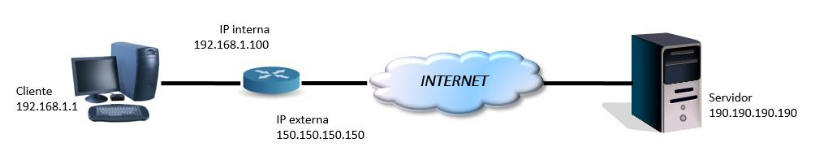
\includegraphics[width=0.7\textwidth]{images/enunciado1ene23.png}
    \caption{Ejemplo de NAT.}
\end{figure}

\subsection{Solución}

\subsubsection{Explicación de NAT}
El \textbf{Network Address Translation (NAT)} permite traducir direcciones IP privadas a direcciones IP públicas (y viceversa) para habilitar la comunicación entre una red interna y una red externa, como Internet.

\begin{itemize}
    \item \textbf{SNAT (Source NAT):} 
    Se utiliza cuando un cliente está en la red privada y necesita comunicarse con un servidor en Internet. La dirección IP privada y el puerto de origen del cliente se traducen a la dirección IP pública del router y un puerto asignado dinámicamente por el router. Esto asegura que múltiples clientes de la red privada puedan compartir la misma dirección IP pública.
    \item \textbf{DNAT (Destination NAT):} 
    Se utiliza cuando un cliente externo necesita acceder a un servidor en la red privada. La dirección IP pública y el puerto de destino del paquete se traducen a la dirección IP privada y el puerto del servidor en la red interna.
\end{itemize}

\subsubsection{Ejemplo de Traducción con Tabla}

Supongamos una red con los siguientes elementos:
\begin{itemize}
    \item IP privada del cliente: 192.168.1.100
    \item Puerto privado del cliente: 5000
    \item IP pública del router: 203.0.113.1
    \item Puerto asignado dinámicamente por SNAT: 60001
    \item IP privada del servidor: 192.168.1.200
    \item Puerto privado del servidor: 80
    \item IP pública del servidor visible en Internet (tras DNAT): 203.0.113.2
\end{itemize}

\begin{table}[H]
    \centering
    \begin{tabular}{|c|c|c|p{5cm}|}
        \hline
        \textbf{Tipo de NAT} & \textbf{IP y Puerto de Origen} & \textbf{IP y Puerto de Destino} & \textbf{Traducción}\\
        \hline
        \textbf{SNAT} & 192.168.1.100:5000 & 198.51.100.10:80 & 203.0.113.1:60001 → 198.51.100.10:80\\
        \hline
        \textbf{DNAT} & 203.0.113.2:80 & 192.168.1.200:80 & 203.0.113.2:80 → 192.168.1.200:80\\
        \hline
    \end{tabular}
    \caption{Ejemplo de traducción con SNAT y DNAT}
\end{table}

\textbf{Nota:} En SNAT, el puerto de origen se traduce para evitar conflictos si varios clientes de la red privada usan el mismo puerto. En DNAT, la dirección pública y el puerto son mapeados al servidor interno correspondiente.

\begin{figure}[H]
    \centering
    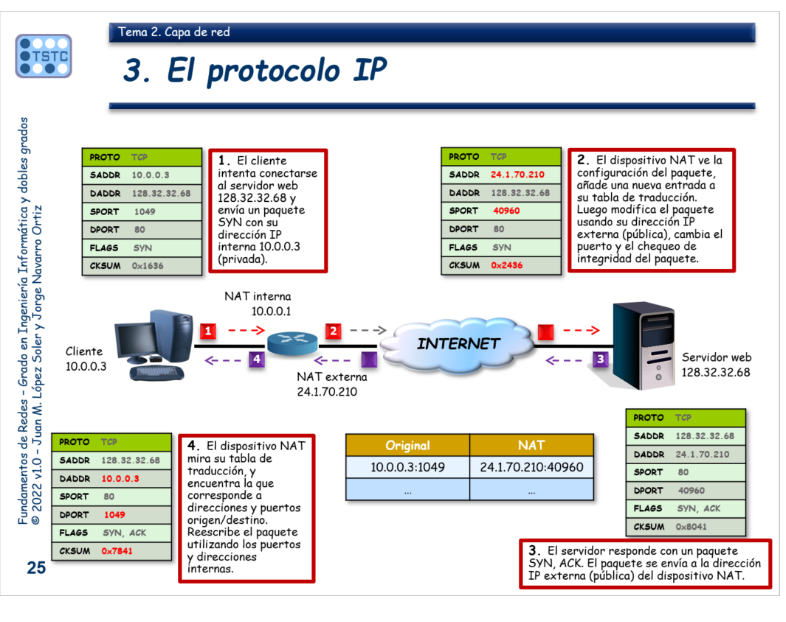
\includegraphics[width=0.7\textwidth]{images/NAt.png}
    \caption{Ejemplo de NAT con traducción de direcciones IP y puertos.}
\end{figure}


\section{Pregunta 2}

\subsection{Enunciado}
Muestre con un ejemplo el uso de cifrado asimétrico (KPUB\_A / KPRIV\_A y KPUB\_B / KPRIV\_B) para garantizar el no repudio en una transmisión entre A y B. Explique qué requisitos deben cumplir las claves para asegurar el no repudio. Justifique su respuesta.

\subsection{Solución}
El ejemplo de cifrado asimétrico para garantizar el no repudio en una transmisión entre A y B es el siguiente:

\begin{enumerate}
    \item El usuario A desea enviar un mensaje a B y garantizar el no repudio. Para ello:
    \begin{itemize}
        \item A genera un hash del mensaje (por ejemplo, utilizando SHA-256).
        \item A cifra el hash del mensaje utilizando su clave privada \( KPRIV\_A \), generando una firma digital.
        \item A envía a B el mensaje original junto con la firma digital.
    \end{itemize}
    \item Cuando el usuario B recibe el mensaje:
    \begin{itemize}
        \item B utiliza la clave pública de A \( KPUB\_A \) para descifrar la firma digital y obtener el hash original generado por A.
        \item B calcula nuevamente el hash del mensaje recibido y lo compara con el hash obtenido de la firma digital.
        \item Si ambos hashes coinciden, se asegura que el mensaje fue enviado por A y no ha sido modificado, garantizando el no repudio.
    \end{itemize}
\end{enumerate}

\textbf{Requisitos de las claves para garantizar el no repudio:}
\begin{itemize}
    \item La clave privada \( KPRIV\_A \) debe ser conocida únicamente por A y estar protegida contra accesos no autorizados.
    \item La clave pública \( KPUB\_A \) debe ser accesible públicamente y estar asociada de manera verificable con la identidad de A.
    \item Un tercero confiable (como una autoridad certificadora) debe garantizar la autenticidad de la clave pública \( KPUB\_A \), vinculándola con A mediante un certificado digital.
\end{itemize}

\textbf{Justificación:}
El no repudio se logra porque únicamente A, como poseedor de \( KPRIV\_A \), puede haber generado la firma digital. Si B puede verificarla con \( KPUB\_A \), queda garantizado que A fue el emisor del mensaje. Adicionalmente, el uso de un hash asegura que cualquier alteración en el mensaje original invalidará la firma, proporcionando integridad.

\subsection{Solución propia del examen y de las diapositivas}

Respuesta sencilla: usar doble cifrado (véase la transparencia debajo) y faltaría incluir que es necesario
garantizar la relación entre la identidad del emisor y su clave pública. Para ello, necesitamos una entidad
en la que todos confiemos y que lo garantice $\rightarrow$ eso es precisamente lo que hacen los certificados digitales,
incluyen la identidad, la clave pública, más datos, y lo firman todo con la clave privada de la autoridad de
certificación (en quienes todos confían). Con eso se consigue el no repudio. Se debería incluir también un
resumen (hash) para conseguir integridad, algo necesario en la firma digital.

\begin{figure}[H]
    \centering
    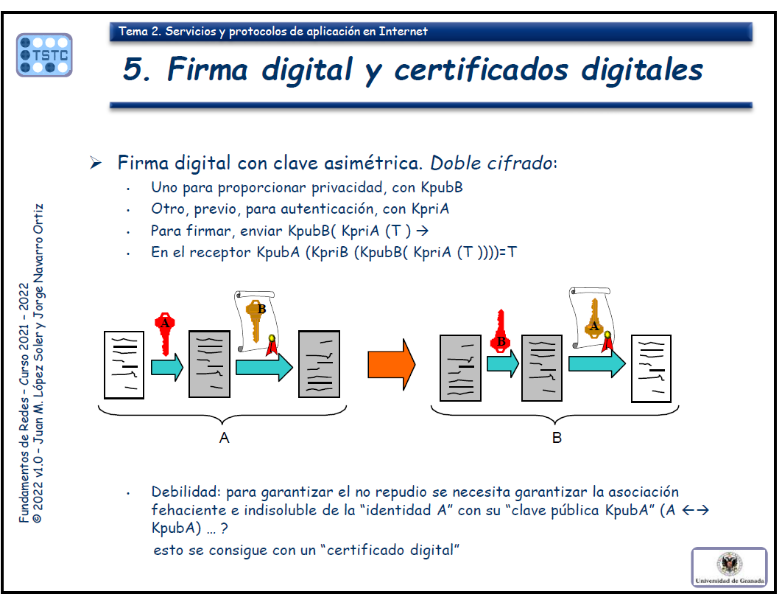
\includegraphics[width=0.7\textwidth]{images/pregunta2Examenene23.png}
    \caption{Doble cifrado para garantizar el no repudio.}
\end{figure}



\section{Pregunta 3}

\subsection{Enunciado}
Explique qué condición se debe cumplir entre el tiempo de transmisión, el tiempo de propagación y el tamaño de la ventana de congestión en un emisor TCP para que no haya interrupción (paradas) en la transmisión.  

Para que no haya interrupciones, desde que mandamos un paquete hasta que nos llega su ACK debemos estar enviando siempre paquetes (sin que la ventana de congestión, CW, nos limite).

\subsection{Solución}
1) \textbf{Tiempo desde que mandamos un paquete hasta que llega su ACK:}  
\[ RTT = 2 \cdot T_t + 2 \cdot T_p \]  
donde:  
\begin{itemize}
    \item \( T_t \) es el tiempo de transmisión.
    \item \( T_p \) es el tiempo de propagación.
\end{itemize}  
El factor \( 2 \cdot T_t \) incluye el tiempo necesario para enviar dos paquetes TCP (uno de datos y otro de ACK). Esto evita interrupciones debidas a tiempos adicionales de espera.

2) \textbf{Tiempo que tardamos en mandar una ventana entera:}  
\[ T_{\text{ventana}} = CW \cdot T_t \]  
donde:  
\begin{itemize}
    \item \( CW \) es el tamaño de la ventana de congestión.
    \item \( T_t \) es el tiempo de transmisión por paquete.
\end{itemize}

3) \textbf{Condición para evitar interrupciones:}  
Para evitar interrupciones en la transmisión, el tiempo de ida y vuelta (\( RTT \)) debe ser menor o igual al tiempo necesario para transmitir una ventana completa:  
\[ 2 \cdot T_t + 2 \cdot T_p \leq CW \cdot T_t \]

\begin{figure}[H]
    \centering
    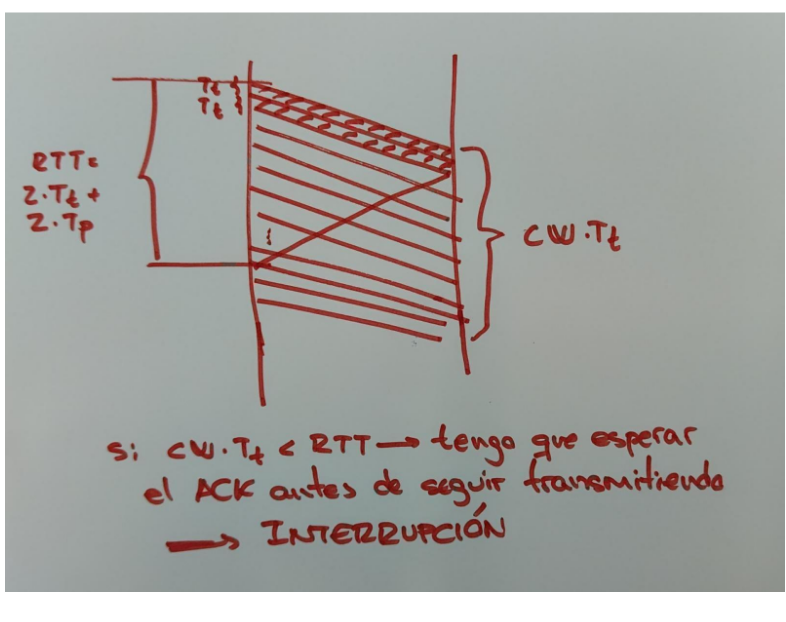
\includegraphics[width=0.7\textwidth]{images/pregunta3ene23.png}
    \caption{Condición para evitar interrupciones en la transmisión.}
\end{figure}


%incluye las paginas 5,6,7 de un pdf
\includepdf[pages=3-7]{../../Examenes_Prado/fr-teoria-feb22 - extraordinaria - resuelto.pdf}

\includepdf[pages=5-6]{../../Examenes_Prado/fr-teoria-ene22 - solución.pdf}

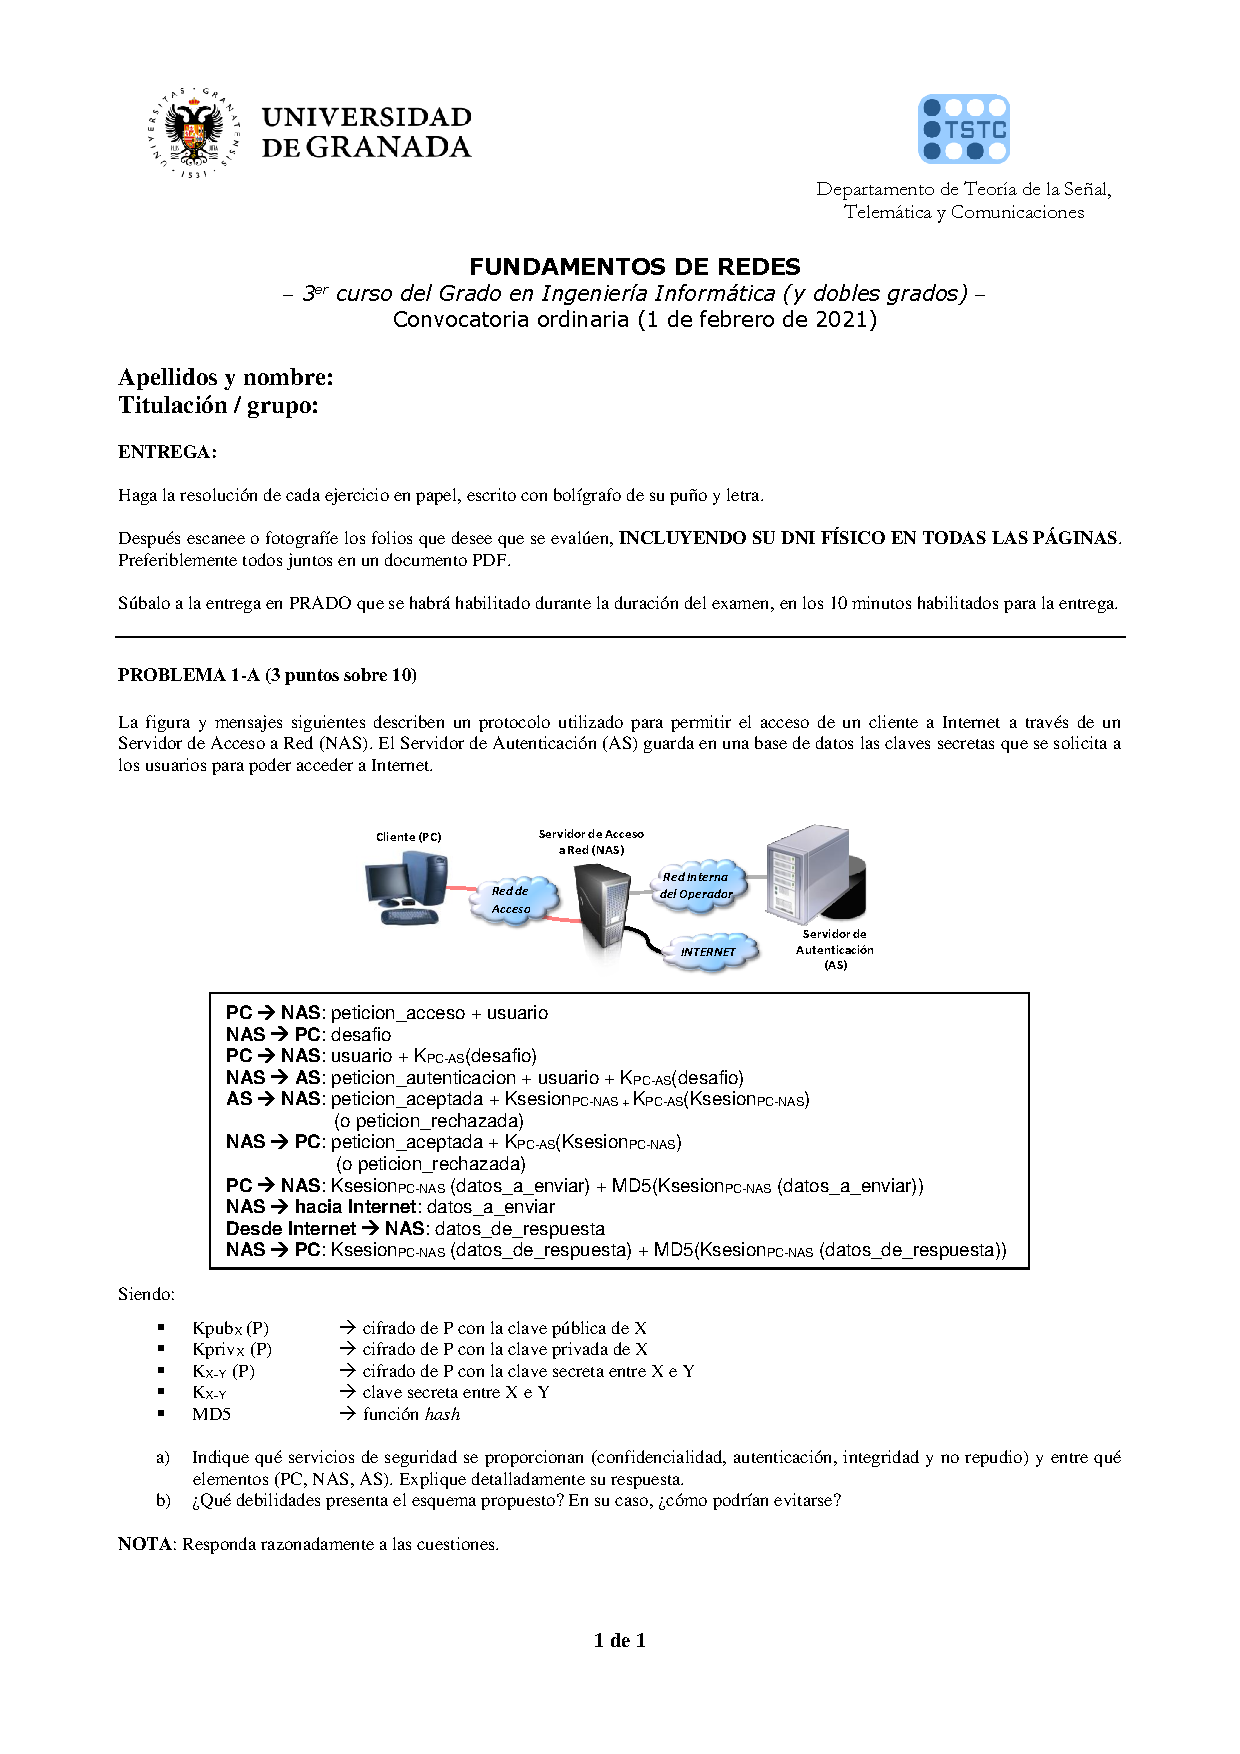
\includepdf[pages=1-3]{../../Examenes_Prado/ENERO_2021.pdf}

\section{Examenes de 2019}

Las preguntas son tipo test, pueden servir para entender conceptos.

%incluye las paginas 5,7 de un pdf
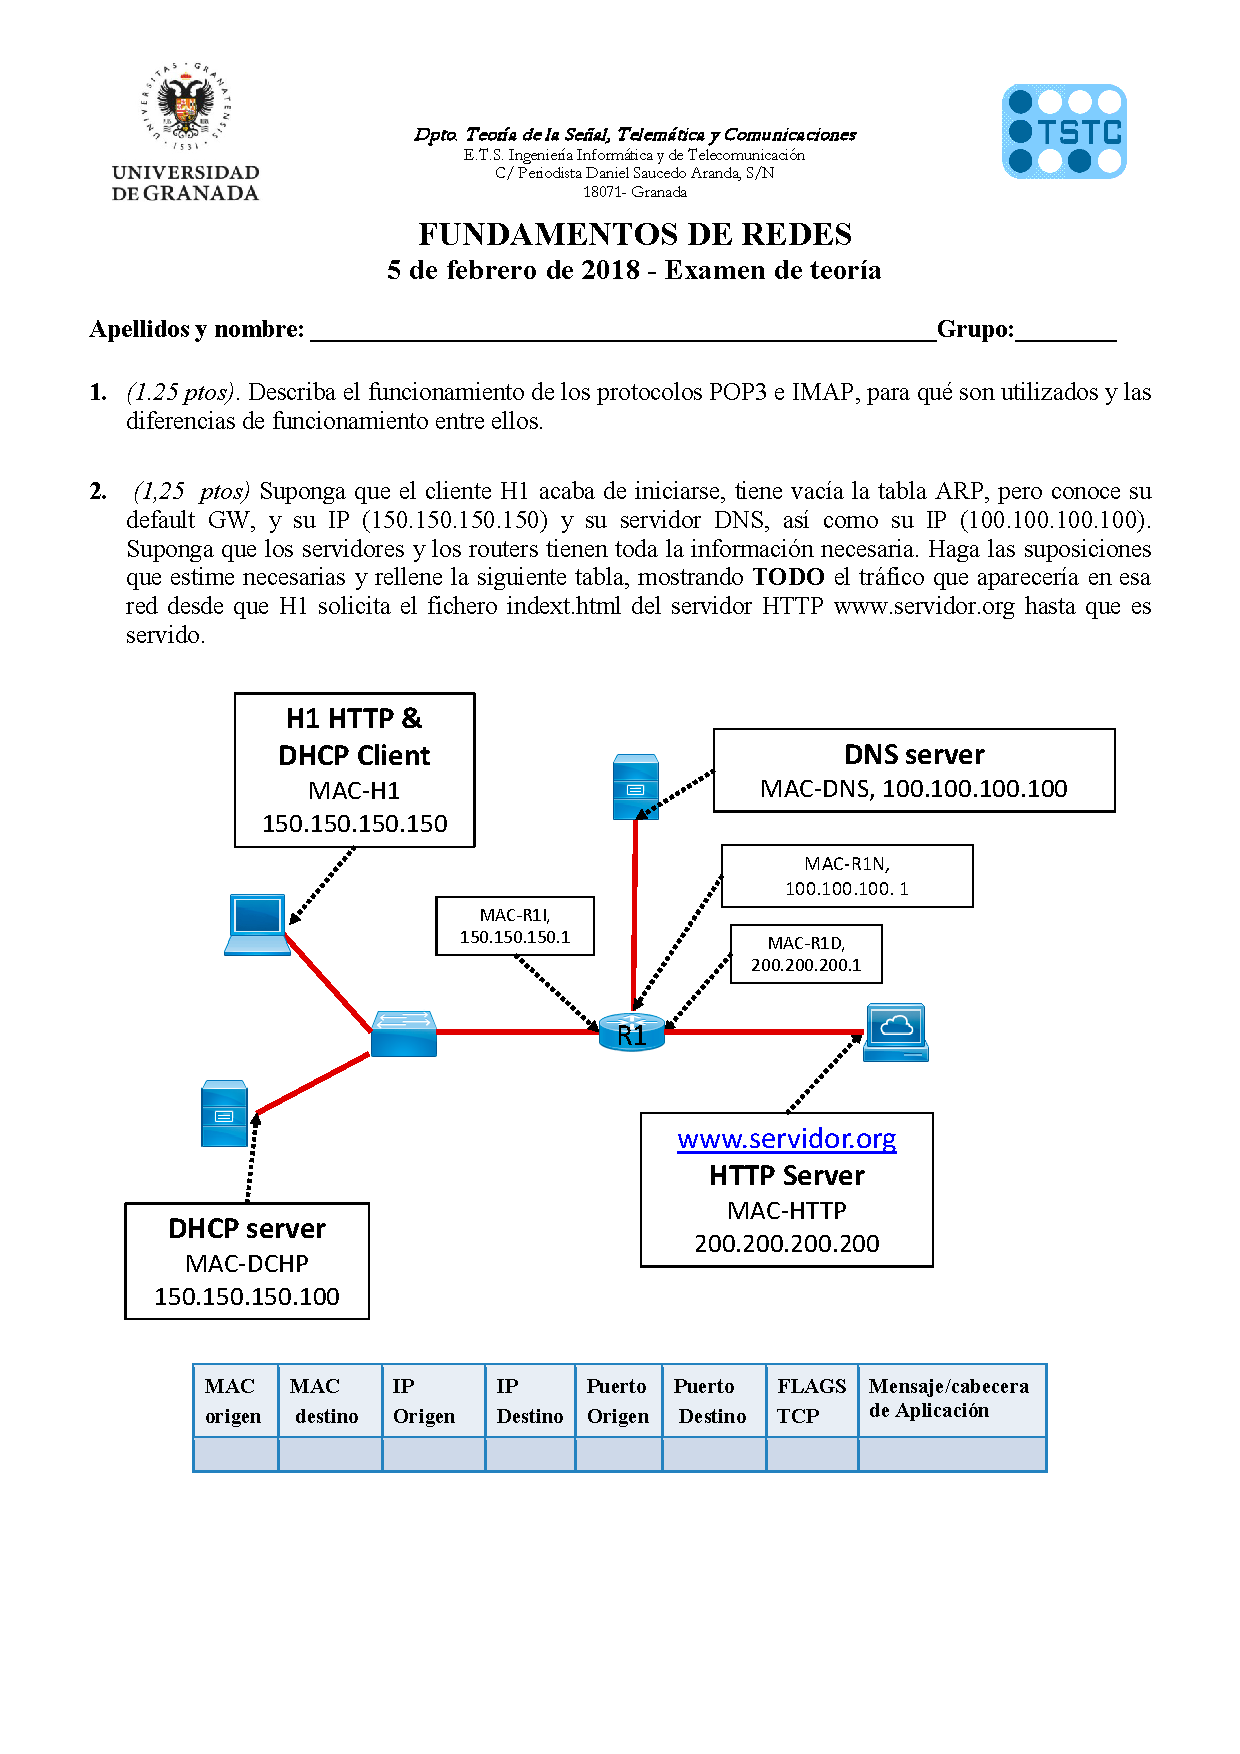
\includepdf[pages={1,3}]{../../Examenes_Prado/FEBRERO_2018.pdf}

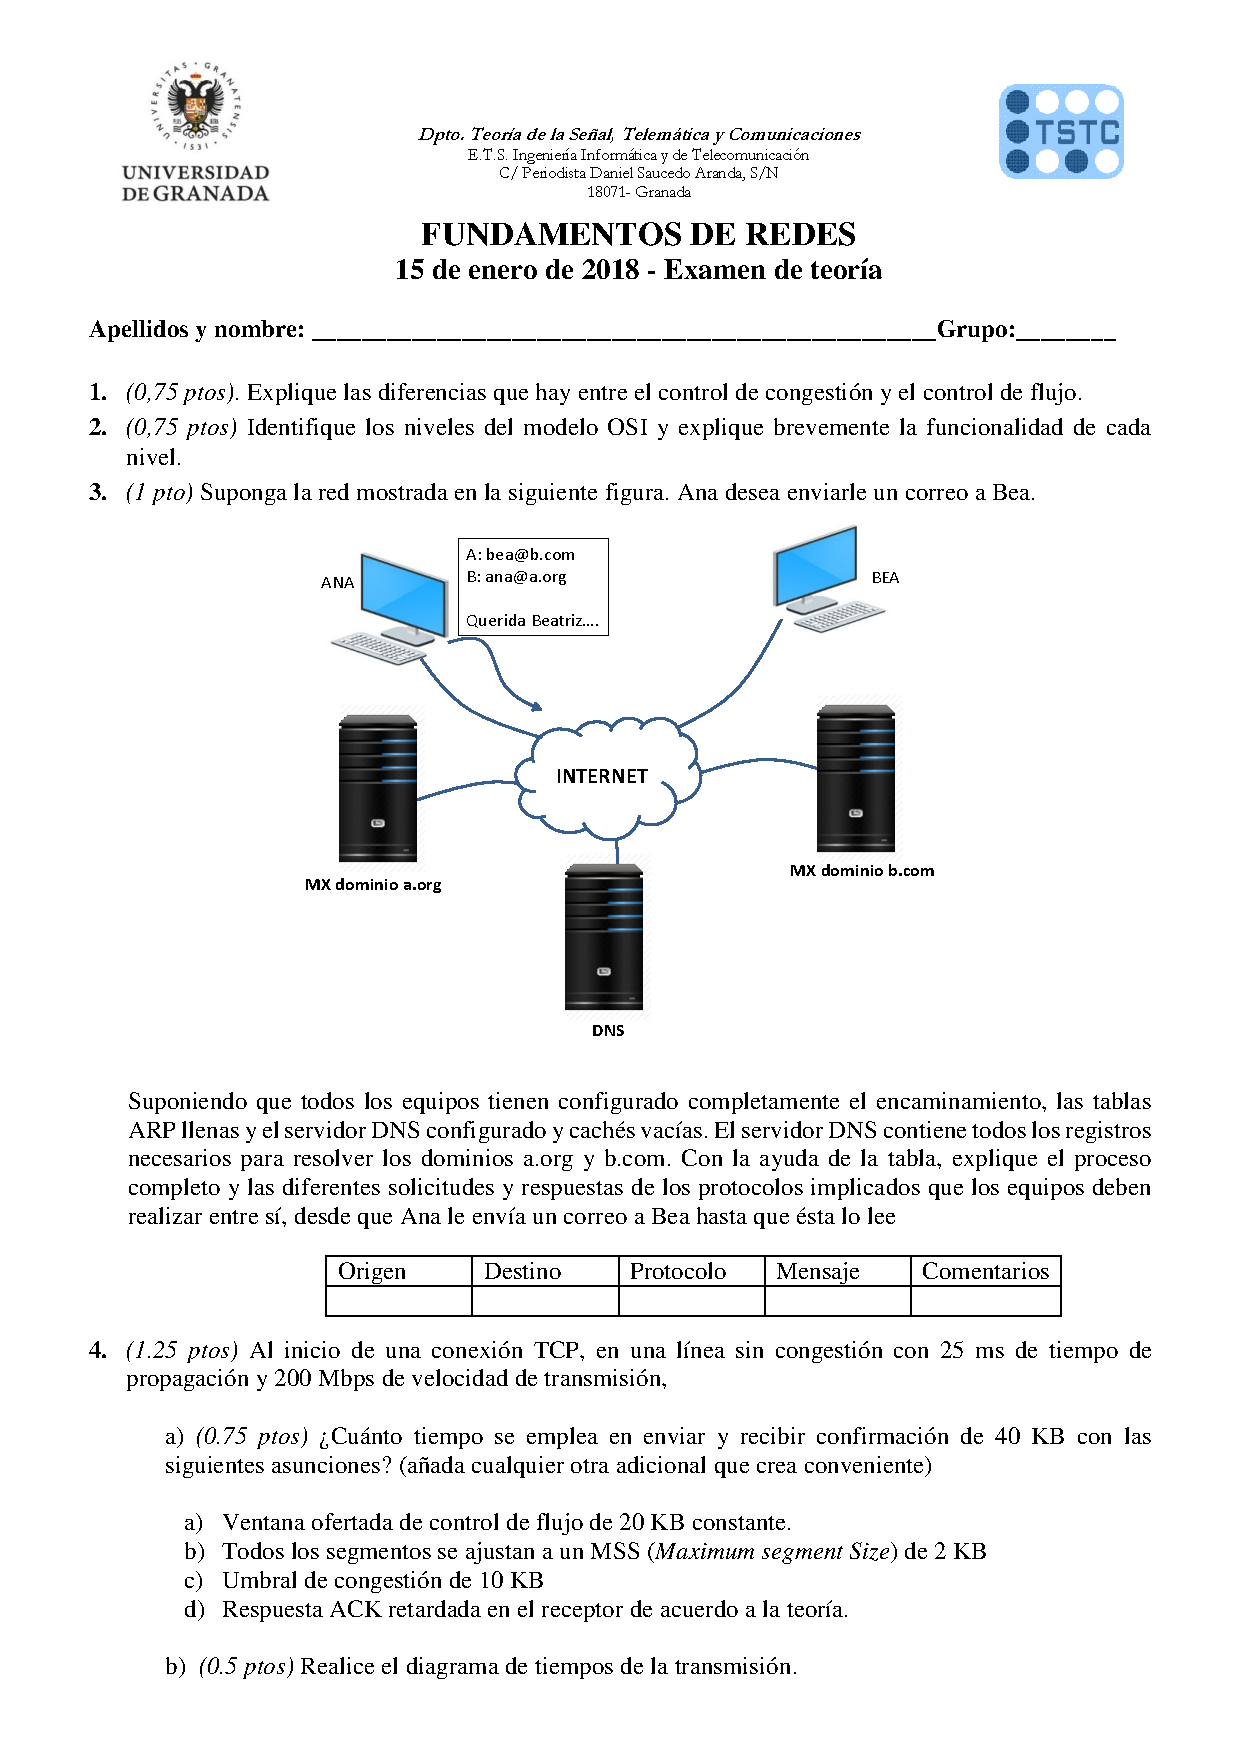
\includepdf[pages={1,3}]{../../Examenes_Prado/ENERO_2018.pdf}

\section{Preguntas Variadas}

\subsection{Pregunta 1 (0,75 puntos)}
\subsubsection{Enunciado}
Describa los mensajes generados desde un equipo correctamente configurado para acceder a Internet desde que solicita una URL en el navegador hasta que se muestra la página web completa.

\subsubsection{Solución}
El dispositivo origen de la conexión genera los siguientes mensajes:  
\begin{enumerate}
    \item \textbf{Solicitud DNS:} Se envía una consulta al servidor DNS para obtener la dirección IP correspondiente al nombre de dominio de la URL.
    \item \textbf{Inicio de conexión TCP (3-way handshake):}  
    \begin{itemize}
        \item Primer segmento contiene únicamente cabeceras con el flag SYN para iniciar la conexión.
        \item Recepción del segmento SYN+ACK del servidor.
        \item Envío de un segmento ACK para completar el handshake.
    \end{itemize}
    \item \textbf{Solicitudes HTTP:}  
    \begin{itemize}
        \item Envío de una solicitud HTTP GET para obtener la página solicitada.
        \item Envío de solicitudes adicionales (en este u otros flujos TCP iniciados previamente) para recuperar los objetos incrustados en la página.
    \end{itemize}
\end{enumerate}

\subsection{Pregunta 2 (0,75 puntos)}
\subsubsection{Enunciado}
Suponga que A y B tienen sus correspondientes \( KPUB\_A \) / \( KPRIV\_A \) y \( KPUB\_B \) / \( KPRIV\_B \), y una autoridad tiene sus \( KPUB\_AUT \) / \( KPRIV\_AUT \). Explique cómo y qué primitivas se cumplirían en una comunicación segura entre A y B usando dichas claves.

\subsubsection{Solución}
Las primitivas de seguridad se implementan de la siguiente manera:  
\begin{itemize}
    \item \textbf{Confidencialidad:}  
    Se utiliza criptografía simétrica para cifrar el tráfico. La clave simétrica es negociada usando criptografía asimétrica, donde cada par usa la clave pública del otro para cifrar la información de la negociación.
    \item \textbf{Responsabilidad y Autenticación:}  
    La clave pública de cada par está asociada a su identidad mediante un certificado digital, firmado por la autoridad certificadora utilizando su clave privada (\( KPRIV\_AUT \)).
    \item \textbf{Integridad:}  
    Para garantizar que los mensajes no sean modificados, cada par firma un resumen (MAC) del mensaje con su clave privada. El receptor verifica la integridad utilizando la clave pública del remitente.
\end{itemize}

\subsection{Pregunta 3 (0,75 puntos)}
\subsubsection{Enunciado}
Se tiene un paquete de 5KB, de los cuales 14 bytes son de cabecera Ethernet, 20 bytes de cabecera IP, y 8 bytes de cabecera UDP. Este paquete debe pasar por una red Ethernet con una MTU de 1514 bytes. Si se precisa su fragmentación, ¿cuántos paquetes se generarían y con qué tamaños?

\subsubsection{Solución}
La fragmentación ocurre en la capa IP. Por lo tanto, el tamaño de la SDU (Service Data Unit) es:  
\[ \text{SDU} = 5 \cdot 1024 \, \text{bytes} - (14 + 20) \, \text{bytes} = 5086 \, \text{bytes} \]  

Cada datagrama puede transportar un máximo de:  
\[ \text{Datos por datagrama} = 1500 \, \text{bytes (MTU)} - 20 \, \text{bytes (cabecera IP)} = 1480 \, \text{bytes} \]  

Por lo tanto:  
\begin{itemize}
    \item Se generan \( \lfloor 5086 / 1480 \rfloor = 3 \) datagramas completos de \( 1480 \, \text{bytes} \) de datos.
    \item El datagrama restante transporta \( 5086 - (3 \cdot 1480) = 646 \, \text{bytes} \).
\end{itemize}

Tamaños de los datagramas:  
\begin{enumerate}
    \item 3 datagramas de \( 1480 + 20 + 14 = 1514 \, \text{bytes} \).
    \item 1 datagrama de \( 646 + 20 + 14 = 680 \, \text{bytes} \).
\end{enumerate}

\subsection{Pregunta 4 (0,75 puntos)}
\subsubsection{Enunciado}
Identifique los niveles del modelo OSI y explique brevemente la funcionalidad de cada nivel.

\subsubsection{Solución}
\begin{enumerate}
    \item \textbf{Nivel de Aplicación:} Brinda servicios a las aplicaciones del usuario (ej., HTTP, FTP).
    \item \textbf{Nivel de Presentación:} Maneja la representación de datos, incluyendo traducción, compresión y cifrado.
    \item \textbf{Nivel de Sesión:} Coordina y mantiene las sesiones entre aplicaciones.
    \item \textbf{Nivel de Transporte:} Proporciona control de errores, control de flujo y multiplexación de aplicaciones (ej., TCP, UDP).
    \item \textbf{Nivel de Red:} Encargado del direccionamiento, enrutamiento y control de congestión (ej., IP).
    \item \textbf{Nivel de Enlace:} Proporciona la delimitación de tramas, control de errores y flujo entre nodos adyacentes.
    \item \textbf{Nivel Físico:} Gestiona la transmisión de datos en forma de señales físicas a través de los medios de comunicación.
\end{enumerate}



\end{document}
